\section{Consenso Promedio en Sistemas Holonómicos}
\onecolumn
\subsection{Agente aislado}
Se anula la percepción de un agente, es decir $\mathbf{u}_1 = 0$. Deja de escuchar a los demás y nunca se mueve, aunque el resto sí lo escucha.

\begin{figure}[H]
    \centering
    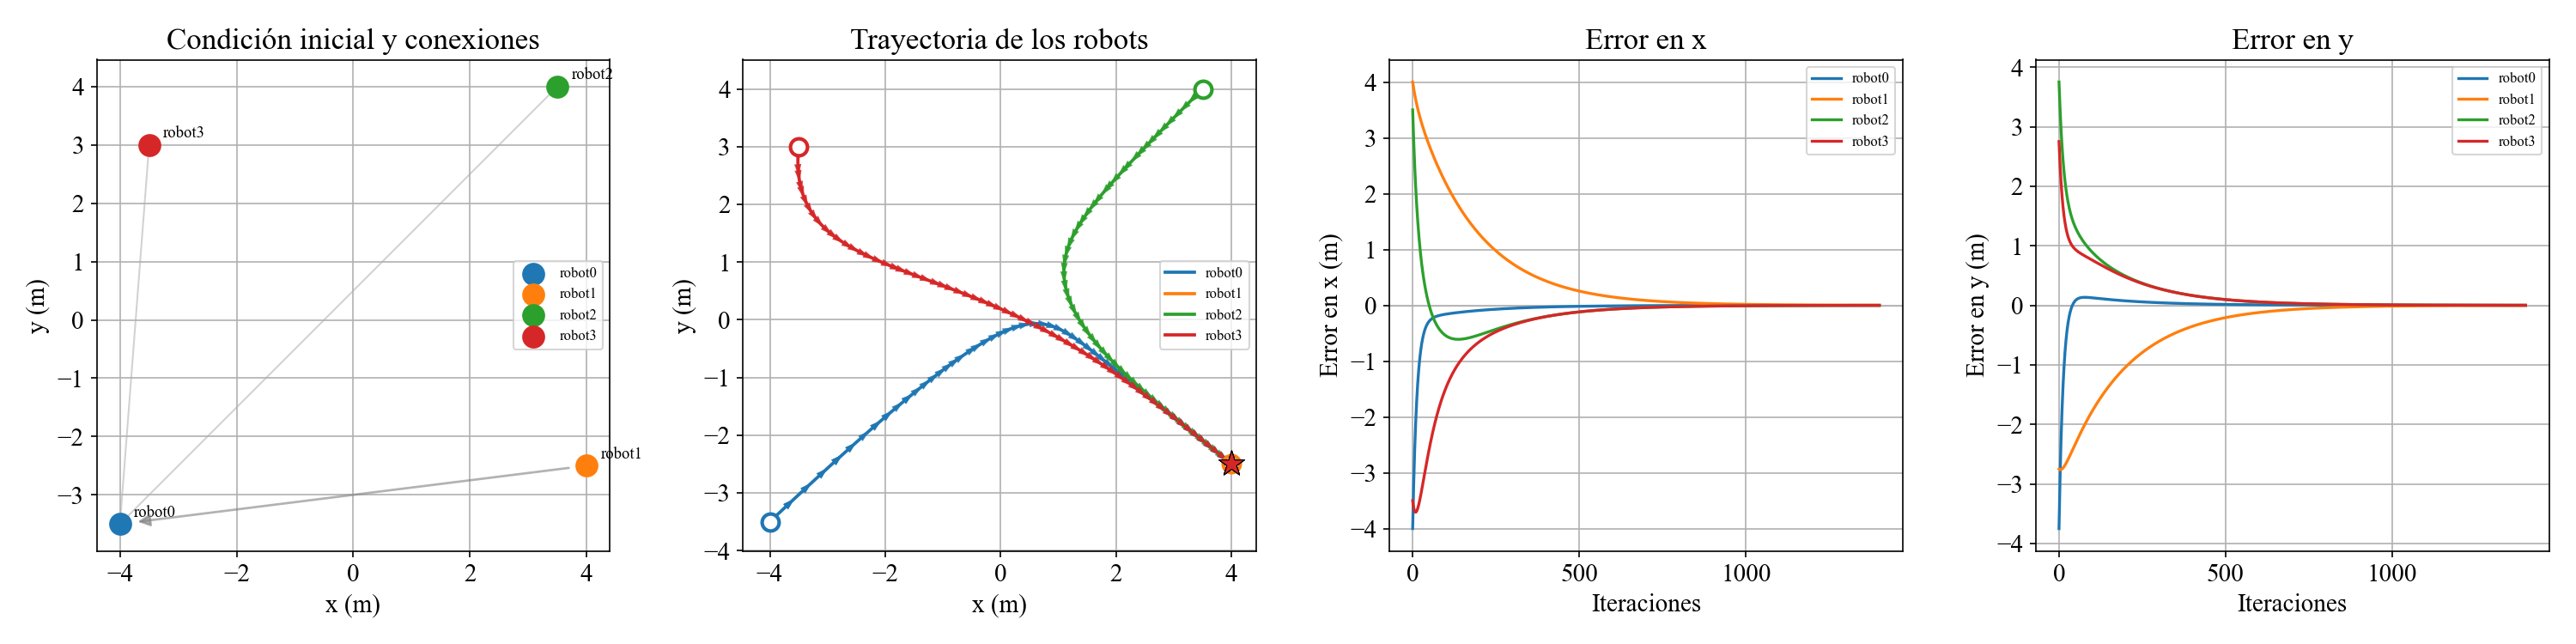
\includegraphics[width=\linewidth]{Pics/consenso_promedio_not (1).png}
    \caption{Al aislar un agente, el resto converge hacia su posición fija en vez del promedio real del grupo.}
    \label{fig:consenso_aislado}
\end{figure}
